% https://tex.stackexchange.com/questions/144577/remove-chapter-number-from-bibliography

\documentclass[
%a4paper, 
11pt, 
ngerman,
listof=totoc,
oneside,
%bibliography=totoc,
bibliography=totocnumbered,
abstracton
]{scrreprt}

\usepackage[T1]{fontenc}
\usepackage[utf8]{inputenc}
\usepackage[ngerman]{babel}
\usepackage{graphicx}
\usepackage{lipsum}
\usepackage{csquotes}
\usepackage[onehalfspacing]{setspace}
\usepackage{scrlayer-scrpage}
\usepackage{float}
\usepackage{mhchem}
\usepackage{siunitx}
\usepackage{pdfpages}
\chead*{\pagemark}
\cofoot*{}

\usepackage{lineno}
%\usepackage{layout}
%
%\makeatletter
%\renewcommand*{\lay@value}[2]{%
%	\strip@pt\dimexpr0.351459\dimexpr\csname#2\endcsname\relax\relax mm%
%}
%\makeatother

\usepackage[a4paper
,showframe
,top=2.5cm
,bottom=2.5cm
,left=3.5cm
,right=2.5cm
]{geometry}

\usepackage[
backend=biber,
style=authoryear-ibid,
%sorting=ynt
]{biblatex}
\addbibresource{gravitropismus-bibliography.bib}

\title{Untersuchung von Gravitropismus bei \emph{Lepidium sativum} mit einem selbstgebauten Klinostat unter Zimmerbedingungen}

\subtitle{W-Seminararbeit im Fach Biologie am Luitpold-Gymnasium München}

\author{Alexandra Smirnova}


\begin{document}
	

\includepdf[pages={1}]{1.pdf}

\begingroup
\renewcommand*{\chapterpagestyle}{empty}
\pagestyle{empty}
% \maketitle
\tableofcontents
\clearpage
\endgroup
	
\renewcommand\abstractname{Abstract}
\begin{abstract}

Gravitropismus ist im 19.Jahrhundert entdeckt worden und ist seit dem ein Thema, das heutzutage ein eigenes Forschungsgebiet darstellt. Allgemein ist bekannt, dass Pflanzen sich nach der Schwerkraft orientieren, um Richtung Licht zu wachsen. Jedoch ist es für das menschliche Auge nicht erkennbar, was für Prozesse und Reaktionen in der Pflanze geschehen. Teile des Mysteriums sind  erforscht, veröffentlicht und stellen das wissenschaftliche Fundament dieser Arbeit dar.

Gravitropismus folgt in drei Schritten ab. Zuerst wird ein verursachter Reiz durch die Statolithen aufgenommen, der in ein Signal umgewandelt wird. Im zweiten Schritt erfolgt dann die Signaltransduktion, wodurch Pflanzenhormone (Auxin oder Gibberelline) aktiviert werden. Diese Hormone führen dazu, dass die Pflanze sich anfänglich krümmt, was den dritten Schritt darstellt.
Diese Bewegung lässt sich experimentell verfolgen.
	
\end{abstract}

% \let\raggedsection\centering
% \section*{\abstractname}
% Dies ist die Zusammenfassung auf Deutsch.

\chapter{Gravitropismus als wichtige Pflanzeneigenschaft}

Viele Pflanzen sind an die Erde festgebundene Organismen, die seit ihrer Keimung ihr ganzes Leben an einem Ort verbringen. Wurzeln verankern die Pflanzen an die Erde und versorgen diese mit Mineralionen und Wasser. Sprossen dagegen wachsen oberhalb der Erde, wo sie Photosynthese betreiben können. Damit Wurzeln und Sprossen von Anfang an in eine abgestimmte Richtung wachsen, sorgt die Fähigkeit, sich nach der Schwerkraft zu orientieren. Diese Fähigkeit wird als Gravitropismus bezeichnet \parencite[2]{Masson2002}. 

Gravitropismus, als Forschungsgebiet, wurde vor zweihundert Jahren anerkannt. 
Es ist gegenwärtig ein aktives Forschungsbereich. Zu diesem Thema werden viele aktuelle Publikationen veröffentlicht. Zum Beispiel beschäftigt sich eine Gruppe von Naturwissenschaftlern mit Gravitropismus in Bezug auf die Landwirtschaft, um das Potenzial der Pflanze auszuschöpfen. Sie ist dafür verantwortlich, dass sich das Gewächs nach einem Unwetter wieder aufrichtet und weiter wächst \parencite[343]{Chen1999}.

Die nachfolgende Arbeit wird sich mit den Fragen beschäftigen, was Gravitropismus ist und inwiefern es sich experimentell nachweisen lässt. Die erste Frage wird im anfänglichem Teil der fachlichen Analyse geklärt und die zweite Frage erläutet das Experiment.

Der erste Teil der Arbeit klärt Fragen zur fachlichen Analyse und der zweite Teil der Arbeit erläutert das Experiment. 




%Mit Anführungszeichen: {\glqq Term mit\grqq} 



\chapter{Fachliche Analyse der Thematik Gravitropismus}

In der vorliegenden Arbeit wird die Theorie des Gravitropismus kurz geklärt und dann im experimentellen Teil nachgewiesen. Zuerst werden für den Gravitropismus grundlegende Begriffe aus der Botanik geklärt, um die Reizaufnahme, die Signaltransduktion und das darauf folgende differenzielles Wachstum besser verstehen zu können.  



\section{ Gravitropismus grundlegende Begriffe aus der Botanik}

\subsection{Morphologie der Pflanze}

Um die Prozesse des Gravitropismus zu verstehen, ist es wichtig den Aufbau der Pflanze zu kennen, um die Vorgänge des Gravitropismus in den verschiedenen Bereichen der Pflanze verfolgen zu können.


\begin{figure}[H]
	\centering 
	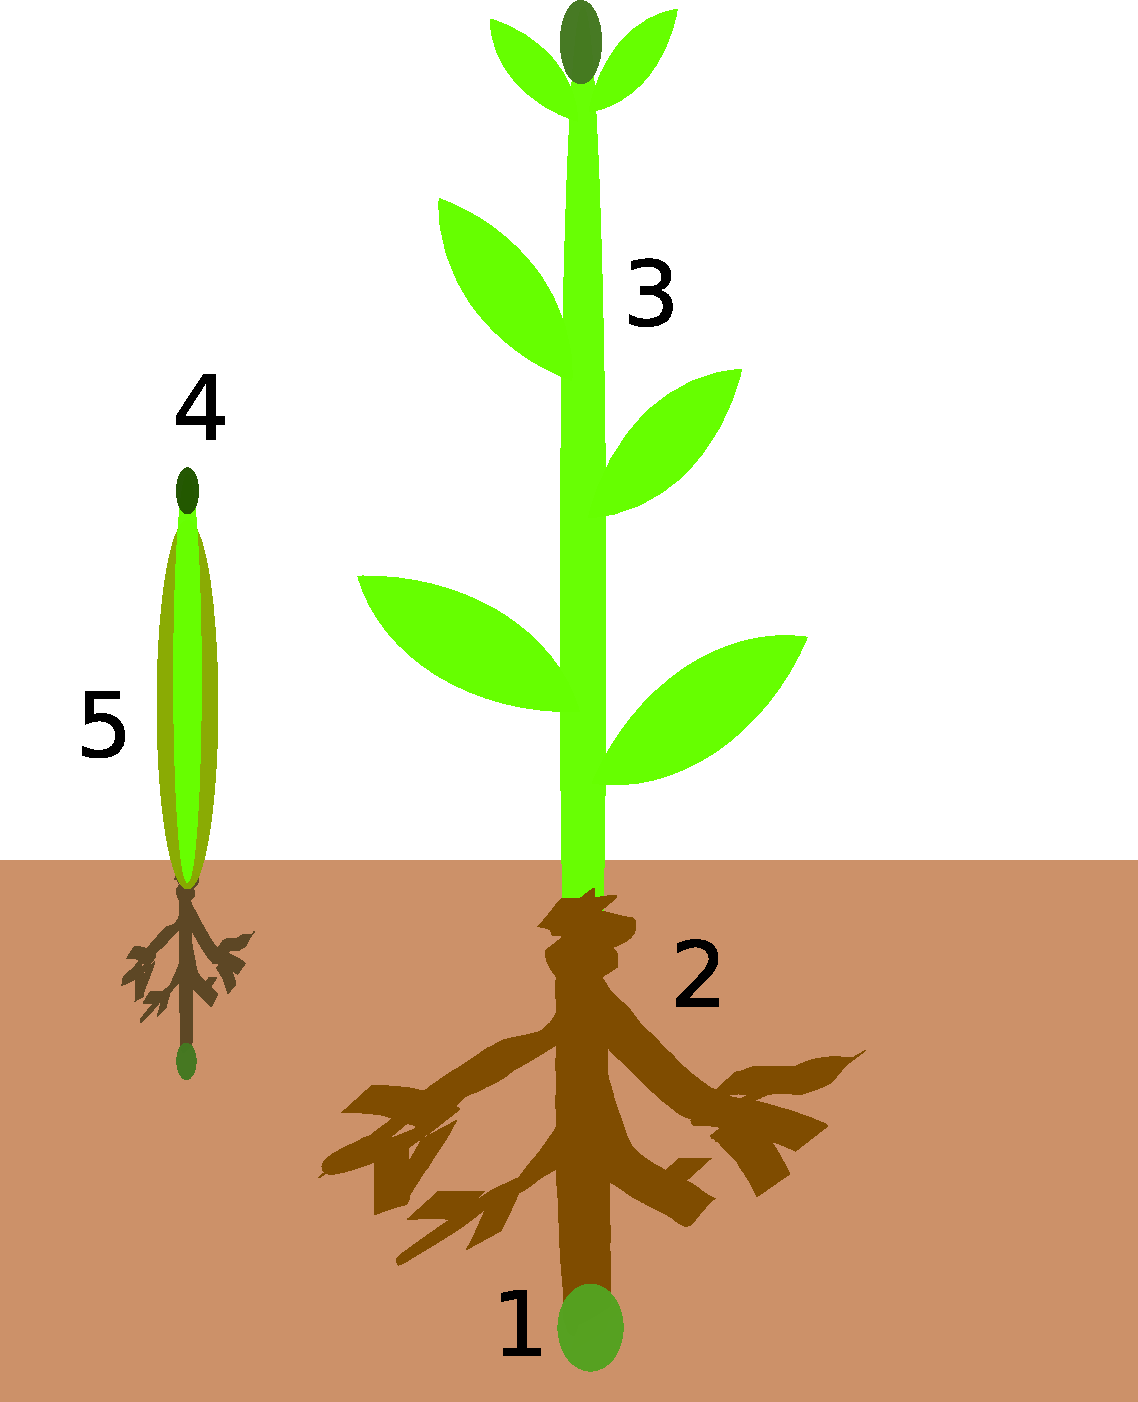
\includegraphics[width = 0.3\linewidth]{images/Spross.pdf}
	\caption{1. Wurzelspitze, 2. Hauptwurzel mit Seitenwurzeln der ersten Ordnung, 3. Sprossachse, 4. Sprossspitze (Apex), 5. Koleoptil (Schutzorgan)}
\end{figure}

Am Anfang der Entwicklung einer Pflanze, wenn sie noch ein Keimling ist, wird sie von einem Schutzorgan, dem \emph{Koleoptil}, umgeben, das sehr sensibel ist. Bei ausgewachsenen Pflanzen ist sie nicht mehr vorhanden. 
Ausgewachsene Pflanzen bestehen aus einer Sprossachse, an der am oberen Ende sich die Sprossspitze (\emph{Apex}) befindet. Am unteren Ende fängt die Hauptwurzel an, von der sich Seitenwurzeln, auch \emph{Adventivwurzeln} genannt, bilden. Am Ende der Hauptwurzel befindet sich die Wurzelspitze, hinter der sich die Streckungszone befindet. An der Sprossspitze sowie an der Wurzelspitze befinden sich Primärmeristeme (Bildungsgewebe). 

\subsection{Arten des Gravitropismus}

Beim Gravitropismus, auch genannt Geotropismus, werden drei Bewegungsarten unterschieden: \emph{Positiv gravitrop},  \emph{negativ gravitrop} und \emph{transversalgravitrop}.
Positiv gravitrop bedeutet, dass das Wachstum der Organe, wie zum Beispiel Wurzeln, Rhizoide (wurzelähnliche Strukturen), Moose oder Farnprothallien, zur Schwerkraftquelle hin (nach unten zur Erdmitte) erfolgt.
Negativ gravitrope Organe dagegen, wie Sprossen, Sporangienträger der Schimmelpilze der Gattung \emph{Mucor} oder Fruchtkörper mancher Pilze wachsen von der Schwerkraftquelle entgegengesetzt (nach oben).

Diese zwei Wachstumsrichtungen werden auch als \emph{Orthogravitropismus} bezeichnet, da sie beide parallel zur Schwerkraft wachsen \parencite[546]{Jacob}.
Seitenwurzeln der ersten Ordnung (Nebenwurzeln, die von der Hauptwurzel entspringen) und zahlreiche Seitenzweige sowie Blätter wachsen \emph{ transversalgravitrop}: entweder horizontal oder quer nach unten in einem bestimmten Winkel \parencite[449]{Strasburger}. 

\begin{figure}[H]
\centering 
 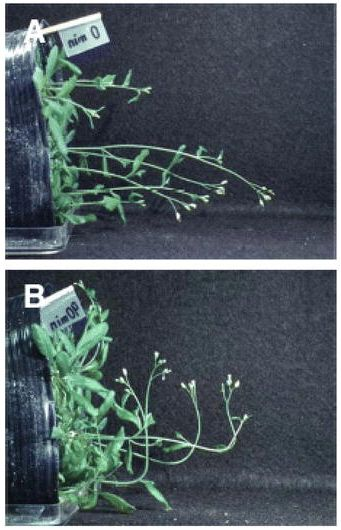
\includegraphics[width = 0.3\linewidth]{images/gravitrop_reagierende_Pflanze.jpg}
 \caption{Gravitrop reagirende \emph{Arabidopsis thaliana} \parencite[5]{Masson2002} \label{gravitrop_reagierende_Pflanze}}
\end{figure} 
 
Legt man eine Pflanze quer, so werden sich Wurzeln und Spross krümmen, bis sie senkrecht stehen und wieder positiv bzw. negativ gravitrop wachsen \parencite[528]{Luettge}, wie in der Abbildung \ref{gravitrop_reagierende_Pflanze}  erkennbar ist.

\section{Reizaufnahme}

Damit eine gravitrope Krümmung entstehen kann, werden zuvor Reize durch \emph{Statolithen}, schwere Körperteilchen oder Organelle in bestimmten Zellen des Sprosses (Abbildung \ref{Statolithen}), der \emph{Koleoptil}-, und der Wurzelspitzen aufgenommen. Es handelt sich dabei meist um \emph{Amyloplasten}, die aus Stärke bestehen \parencite[530]{Luettge}.

\begin{figure}[H]
	\centering 
	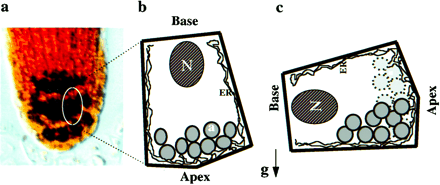
\includegraphics[width = 0.6\linewidth]{images/Statolithen2.png}
	\caption{Statolithen \parencite[345]{Chen1999} \label{Statolithen}}
\end{figure} 

Entscheidend ist der Stärkegehalt  der Amyloplasten, denn ohne ihn geht die gravitrope Reaktionfähigkeit verloren, wobei das Längenwachstum der Wurzeln weiterhin unbeeinflusst bleibt.
Die Stärke aus den Statolithenamyloplasten kann man durch experimentelle Eingriffe, zum Beispiel durch Kühlung, entfernen \parencite[452]{Strasburger}.

Die zahlreich vorhandenen Statolithen befinden sich in Zellen (\emph{Statocysten}), die die Graviperzeption ermöglichen. Kommen Statocysten in größeren Mengen vor, so bilden sie meist ein Gewebe, das als \emph{Statenchyme} bezeichnet wird.
Diese Stärke enthaltenden Bereiche findet man bei den Wurzelhauben und bei Stärkescheiden der Sprossachsen.  
Statolithen üben einen Druck auf Gravisensoren aus, wenn sie von der Schwerkraft beeinflusst werden. Wird die Lage der Pflanzen und ihrer Zellen verändert, so führt dies zu einer Änderung der Druckwirkung, wodurch die Graviperzeption ermöglicht wird \parencite[501--502]{Nultsch}.

 \begin{figure}[H]
 	\centering 
 	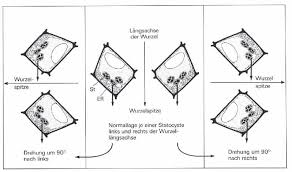
\includegraphics[width = 0.6\linewidth]{images/Graviperzeption.jpeg}
 	\caption{Statolithen und ER-Polster \parencite[533]{Luettge} \label{Graviperzeption}}
 \end{figure} 

Statolithen ruhen auf den {\glqq Polster\grqq} von Membranen des \emph{endoplasmatischen Retikulums} (ER). Dabei haben die Statocysten eine zu den angeordneten ER-Polstern anpassende Form, sodass bei einer Drehung (aus der senkrechten Lage) der Statolithendruck auf das ER der Statocysten auf einer Seite momentan aufgehoben wird: auf der linken Seite bei einer Rechtsdrehung, auf der rechten Seite bei einer Linksdrehung, wie in Abbildung \ref{Graviperzeption} zu sehen ist.
Dadurch erfolgt die Graviperzeption schneller, denn die Verlagerung der Wurzel hängt  mit der Aufhebung des Statolithendrucks auf die ER-Polster links oder rechts der Wurzelhaube zusammen \parencite[531--532]{Luettge}. 

Dies ist aber nur der Fall bei Organen höherer Pflanzen, denn bei einer Einzelzelle, z.B einer \emph{Chara}-Rhizoide, erfolgt die Streckung nur durch Spitzenwachstum (einseitiges Wachstum der Zelle).
\emph{Dictyosomen} (flache, membranumhüllte Hohlräume in der Zelle) synthetisieren dabei Membran- und Zellwandbausteine unter dem Bereich der wachsenden Spitze und transportieren  die entstandenen \emph{Vesikel}.

Vesikel wandern auf der Oberseite, da beim Verlagern der Statolithen auf die Unterseite, der Weg dort damit gesperrt wird. Bei der Oberseite bewirken sie somit ein verstärktes Wandwachstum, also einen positiven Gravitropismus.

Bei gravitrop reagierenden Pilzen werden Amyloplasten durch {\glqq Glanzkörper\grqq} ersetzt, die die Funktion der Statolithen übernehmen, da Pilze keine Stärke enthalten. Diese in \emph{Vacuolen} liegenden Einschlusskörper besitzen einen hohes spezifisches Gewicht, da sie aus \ce{BaSO4} bestehen \parencite[453--454]{Strasburger}.

Zusammengefasst lässt es sich sagen, dass durch die Verlagerung der Statolithen ein Druck auf die ER-Polster verursacht wird, wodurch eine schnellere Graviperzeption ermöglicht wird. Dies ist der Fall bei Organen höherer Pflanzen.
Bei Einzelzellen gibt es nur ein Spitzenwachstum, dass durch die Verlagerung der Glaskörperchen, die die Funktion der Statolithen ersetzen, hervorgerufen wird.




\section{Signaltransduktion und differenzielles Wachstum}

\subsection{Teilnahme des Calciums bei der Signaltransduktion}

Die Signalübermittlung durch den direkten Kontakt zwischen Amyloplasten und ER wird als \emph{gravisensorische Transduktion} bezeichnet.
Durch den Druck der Amyloplasten auf die ER-Membranen wird ein \ce{Ca^{2+}}-Efflux (das Austreten von Molekülen oder Ionen an der Zellmembran) aus dem ER verursacht.
Dadurch wird die lokale \ce{Ca^{2+}}-Konzentration im  \emph{Cytoplasma} erhöht. 
Bereits ein Druck auf eine einzige ER-Zysterne reicht aus, um einen Efflux zu verursachen.

\subsection{Teilnahme des Elektronischen Feldes bei der Signaltransduktion}

Wichtiger bei der Signalumwandlung sind jedoch die Änderungen des elektrischen Feldes, dass die Wurzel umgibt.
Bei senkrecht stehenden Pflanzen wandern positive geladene Ionen (hier: Protonen) in die Wurzelspitze ein und treten im Bereich der Zellstreckzone wieder aus.

Diese Ionenbewegung wird als apoplastischer Strom bezeichnet, der das elektrisches Feld, das die Wurzel umgibt, erzeugt. Dieses Feld ist mit einer hochempfindlichen Vibrationselektrode nachweisbar. 
Wird die Pflanze horizontal gelegt, so werden die Wurzeln gravitropisch gereizt. Dabei gelangen die Protonen nur noch in die untere Flanke der Wurzelspitze hinein und auf der Oberseite hinaus, wodurch sich das elektrische Feld ändert \parencite[502--503]{Nultsch}.

Dieses durch der Graviperzeption entstandene Signal kann nur in der Streckungszone hinter der Wurzelspitze aufgenommen werden. Kommt das Signal an, so setzt die Krümmung ein, indem die Flanken anfangen, ungleich zu wachsen. Damit ist feststellbar, dass der Perzeptions- und Reaktionsort getrennt sind.

\begin{figure}[H]
	\centering 
	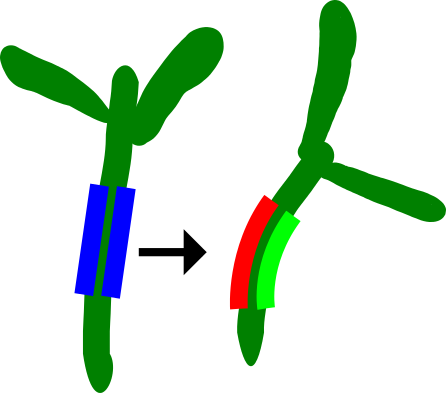
\includegraphics[width = 0.4\linewidth]{images/diff.png}
	\caption{Flanken wachsen ungleich nach der Signaltransduktion. Linkes Bild: Flanken gleich groß (blau); rechtes Bild: unterschiedliche Größe der Flanken (rot und grün).}
\end{figure} 


Für diese Reaktion sind Präsentationszeiten(?) des Reizes wichtig. Sie liegen meist zwischen 2 und 85 Minuten. Das dauert viel länger, als die kürzesten Reizeinwirkungen, die noch wahrgenommen werden können und unter 30 Sekunden liegen. 
Somit wird bei jeder kleinen und kurzen Reizeinwirkung eine Vollführung der Krümmungsbewegung vermieden. Das ist wichtig für Pflanzen, um zum Beispiel eine gravitropische Reaktion auf eine Windeinwirkung zu verhindern \parencite[531]{Luettge}.


\subsection{Funktion der Auxine im Gravitropismus}

Die Ursache der Krümmung nach dem Signal ist die durch Schwerkraft hervorgerufene asymmetrische Verteilung des \emph{Auxins}  \parencite[502--503]{Nultsch}.

Auxin ist ein Pflanzenhormon, das viele Funktionen besitzt. Dabei ist die Stimulierung der Zellstreckung (nur in niedriger Konzentration) und die Seiten- und Adventivwurzelbildung (nicht aus einer apikalen (an der Sprossspitze) oder einem basalen (Wurzel) Primärmeristem entstehend), besonders wichtig. 
Bei Pflanzen ist das natürliche Auxin die Indolessigsäure (IAA), aber alle Verbindungen, die zu einer Streckung von Koleoptilen führen, können als Auxin bezeichnet werden.
Andere Funktionen dieses Hormons wären die Regulierung der Fruchtentwicklung, Verstärkung der Apikaldominanz, Verzögerung der Blattfalls und Förderung der Leitgewebedifferenzierung.

Beim Krümmungsprozess wird Auxin von dee nur in eine Richtung direkt durch das \emph{Parenchymgewebe} (Gewebe, dessen Zellen nebeneinander liegen) transportiert: Von der Sprossspitze längs der Sprossachse bis zur Basis(normal Satz machen). Dieser Transport wird als polarer Transport bezeichnet und ist nicht von der Schwerkraft abhängig.

Auxintransport geschieht durch Auxin-Transportproteinen, die sich am basalen Zellenende befinden, befinden.
Das Hormon wird zur Nachbarzelle am Apikalende transportiert.  durch diese Proteine hinausbefördert.

Auxine werden im Apikalmeristem der Sprossachse synthetisiert. Von dort aus bewegen sie sich zur Streckungszone und stimulieren dabei das Zellwachstum.
Jedoch ist diese Stimulierung nur dann möglich, wenn der Konzentrationsbereich des Auxins zwischen $10^{-8}$ bis $10^{-4}$ \si{\mole\per\L}. Bei höherer Konzentrationen kann Auxin die Zellstreckung durch Induktion der Ethylenbildung hemmen.

Bei der Wachstumsantwort der Zelle auf Auxin spielen Protonenpumpen eine entscheidende Rolle. Das Auxin stimuliert die Protonenpumpen der Plasmamembranen. Es werden Protonen herausgepumpt, wodurch eine Erhöhung des Membranpotenzials entsteht und der pH-Wert in der Zellwand gesenkt wird. 

Durch die Ansäuerung  der Zellwand werden Expansine, spezifische keilförmige Proteine, aktiviert, die die Zellwandstruktur auflockern, indem sie Wasserstoffbrückenbindungen zwischen Cellulosemikrofibrillen und anderen Zellwandbestandteilen lösen.

Das erhöhte Membranpotenzial führt zur erhöhten Ionenaufnahme in die Zelle und damit zur Erhöhung des osmotischen Drucks (\emph{Turgor}). Da die Zellwand plastisch ist, kann sich die Zelle nun ausdehnen. 

Auch die Genexpression wird von Auxin sehr stark beeinflusst, sodass neue Proteine von den Zellen in der Streckungszone gebildet werden.
Außerdem müssen Zellen mehr Cytoplasma und Zellwandmaterial bilden, da das Wachstum aufrecht erhalten werden muss. Dies wird auch durch Auxin stimuliert \parencite[1118ff]{campbell}.

Bei manchen Pflanzenarten (z.B. bei Sonnenblumen \emph{Helianthus} oder Bohnen \emph{Phaseolus}) spielt Auxin jedoch eine untergeordnete Rolle.
Die Steuerung der Krümmung dieser Pflanzenarten übernehmen Gibberelline \parencite[502--503]{Nultsch}.
 
\subsection{Funktion der Gibberelline im Gravitropismus}

\emph{Gibberelline} sind, wie Auxin, Pflanzenhormone und besitzen mehrere Funktionen. 
Sie stimulieren die Sprossstreckung, beeinflussen Pollenentwicklung und sind für Pollenschlauch- und Fruchtwachstum sowie Samenentwicklung und Keimung verantwortlich. Außerdem bestimmen sie das Geschlecht in eingeschlechtigen Blüten und regulieren den Übergang von Jugendphasen zu Adultphasen. 
Bei der Zellstreckung wirken Gibberelline mit Auxin zusammen. Gibberelline aktivieren Enzyme, die die Zellwand auflockern und Expansinen (Proteine) den Eintritt in die Zellwand erleichtern \parencite[1122--1123]{campbell}.

 
Wie dargelegt, ist Gravitropismus ein lebenswichtiges Resultat eines komplexen und zum Teil noch unerforschten Zusammenspiels von biologischen Akteuren. Dennoch lässt sich die gesamte Kaskade mit einfachen Mitteln einleiten und kontrollieren, was zum experimentellen Teil der vorliegenden Arbeit führt. 



\chapter{Experimenteller Nachweis von Gravitropismus bei \emph{Lepidium sativum}}

\section{Methoden}

\subsection{\emph{Lepidium sativum} - Kresse}

Für das Experiment wurde die \emph{Lepidium sativum} (Kresse) genommen. Sie ist eine schnellwüchsige Pflanze und kann auf jedem lockeren, durchlässigen Gartenboden wachsen (der Firma Kiepenkerl).


\subsection{Materialien und Geräte}

Außer den Pflanzen werden vier gleich große Behälter und ein Säckchen, eine Plastiktüte, ein Messzylinder (in mL) und Gegenstände für Stützung der Behälter (z.B. Holzklotz) verwendet.

Für die Pflanzen wurden Anzucht-Quelltabs der Firma Windhager benutzt, da die Erde keinen Torf beinhaltet und Kokosfasern enthält, die dafür sorgen, dass die Feuchtigkeit besser aufgenommen wird.

Samen können dadurch schneller keimen und Wurzeln sich besser ausbilden, wodurch das Wachstum der Pflanze gefördert wird \parencite{Windhager}. 

Für die Aufnahme des ganzen Experimentes wurde eine Kamera (Canon) verwendet.


\subsubsection{Klinostat}

 \begin{figure}[H]
 	\centering 
 	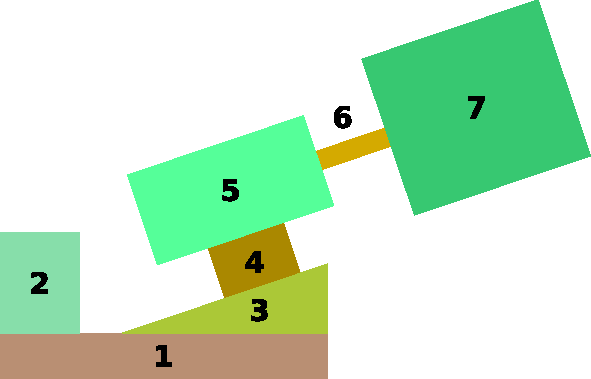
\includegraphics[width = 0.5\linewidth]{images/drawing-1.pdf}
 	\caption{1) Befestigungsplatte (Holz, Dicke: 2cm) 2) Netzteil (Modell: MW1000GS, Eingang: 230V~50Hz 28W, Ausgang: 3-6-9-12V, 1000mA 12VA(max)) 3) Holzkeil, um die Drehachse des Motors um ca. \ang{15} senkrecht zur Ebene anzuheben 4) Motorbefestigung 5) Elektrogetriebemotor MFA/Como Drills 919D SERIES, single ratio gearbox 3000:1 (Untersetzung 3000:1), 4.5 - 15V DC	6) Elektromotorwelle 7) leere Blechdose mit Öffnung (wird mit einer Muffe an die Elektromotorwelle befestigt)}
 \end{figure} 

\subsection{Versuchsbeschreibung}

\subsubsection{Vorbereitung}

Am ersten Tag (28.05.18) wurde für das Experiment vorbereitet: (Ausgewählter Ort: am Fenster) wurde eine Plastiktüte ausgebreitet, um Schmutz auf dem Boden zu vermeiden. Auf die Plastiktüte wurden dann jeder Behälter mit Anzuchterde gefüllt (2/3 der Becher), auf die jeweils 20 Samen, ins Säckchen  nur drei Stück hinzugefügt wurden. Das Säckchen wird später an das Klinostat angebracht. (Im vierten Behälter des Experiments wurden die übrigen Samen eingepflanzt.)


\begin{figure}[H]
	\centering 
	\includegraphics[width = 0.5\linewidth]{images/IMG_1044.JPG}
	\caption{Vorbereitung des Experiments}
\end{figure}


\subsubsection{Durchführung}

Seit dem Tag der Vorbereitung wurden die Pflanzen täglich mit Wasser versorgt (jeweils 20 ml), weitere Bedingungen wie Licht und Wärme wurden konstant gehalten. Ansonsten wurden Veränderungen und Ergebnisse der Pflanzen beobachtet und aufgeschrieben.
Für das Experiment müssen die Pflanzen zuerst stabil wachsen.

Beim ersten Experiment mit dem Klinostat wurde das Säckchen an die Blechdose befestigt. Danach wurde das Klinostat gestartet, dass eine Umdrehung pro Minute vollführte. Zwei Tage später wurde der zweite Versuch gestartet, wo drei Behälter in verschiedenen Positionen gelegt wurden: 1. vertikal zu Boden, 2. Kopfüber, 3. gewinkelt.


\begin{figure}[H]
	\centering 
	\includegraphics[width = 0.5\linewidth]{images/IMG_1376.JPG}
	\caption{Alle Positionen der Behälter}
\end{figure} 


\section{Ergebnisse}

Nach sieben Tagen zeigten die Versuche folgende Ergebnisse:

2.Tag (29.05.18): Die Samen sind gekeimt. 

3. Tag (30.05.18): Sprossen sind ca. 2cm gewachsen (keine Blätter).
Zu diesem Zeitpunkt sind die Sprösslinge nicht geeignet, da die Haftung nicht ausreicht. 

4. Tag (31.05.18): Sprösslinge haben Blätter gebildet und sind geeignet für das Experiment, da ihre Haft nun stabil ist. Der Versuch mit dem Klinostat wird um 12.45 Uhr gestartet (Abbildung \ref{Foto 1}) und um 15.45 gestoppt, da die Sprösslinge gravitrop reagiert haben, wie in der Abbildung \ref{Foto 2} zu sehen ist. Gleichzeitig werden auch die drei Behälter positioniert und beobachtet.

\begin{figure}[H]
	  \centering 
	  \includegraphics[width = .5\linewidth]{images/IMG_1083.JPG}
	  \caption{Sprossen im Originalzustand \label{Foto 1}}
\end{figure}


\begin{figure}[H]
	  \centering 
	  \includegraphics[width = .5\linewidth]{images/IMG_1073.JPG}
	  \caption{Gebogene Sprossen \label{Foto 2}}
\end{figure}



5. Tag (01.06.18): Über Abend haben sich die Pflanzen wieder aufgerichtet wie in Abbildung \ref{Foto 3} zu sehen ist, deshalb war es möglich einen zweiten Durchlauf zu machen, aber um 12:53 (des nächsten Tages) wurde das Klinostat kaputt gefunden. Pflanzen haben aber angefangen sich sichtbar zu biegen (gelaufene Zeit ca. 1 Stunde und 8 Minuten).

\begin{figure}[H]
	\centering 
	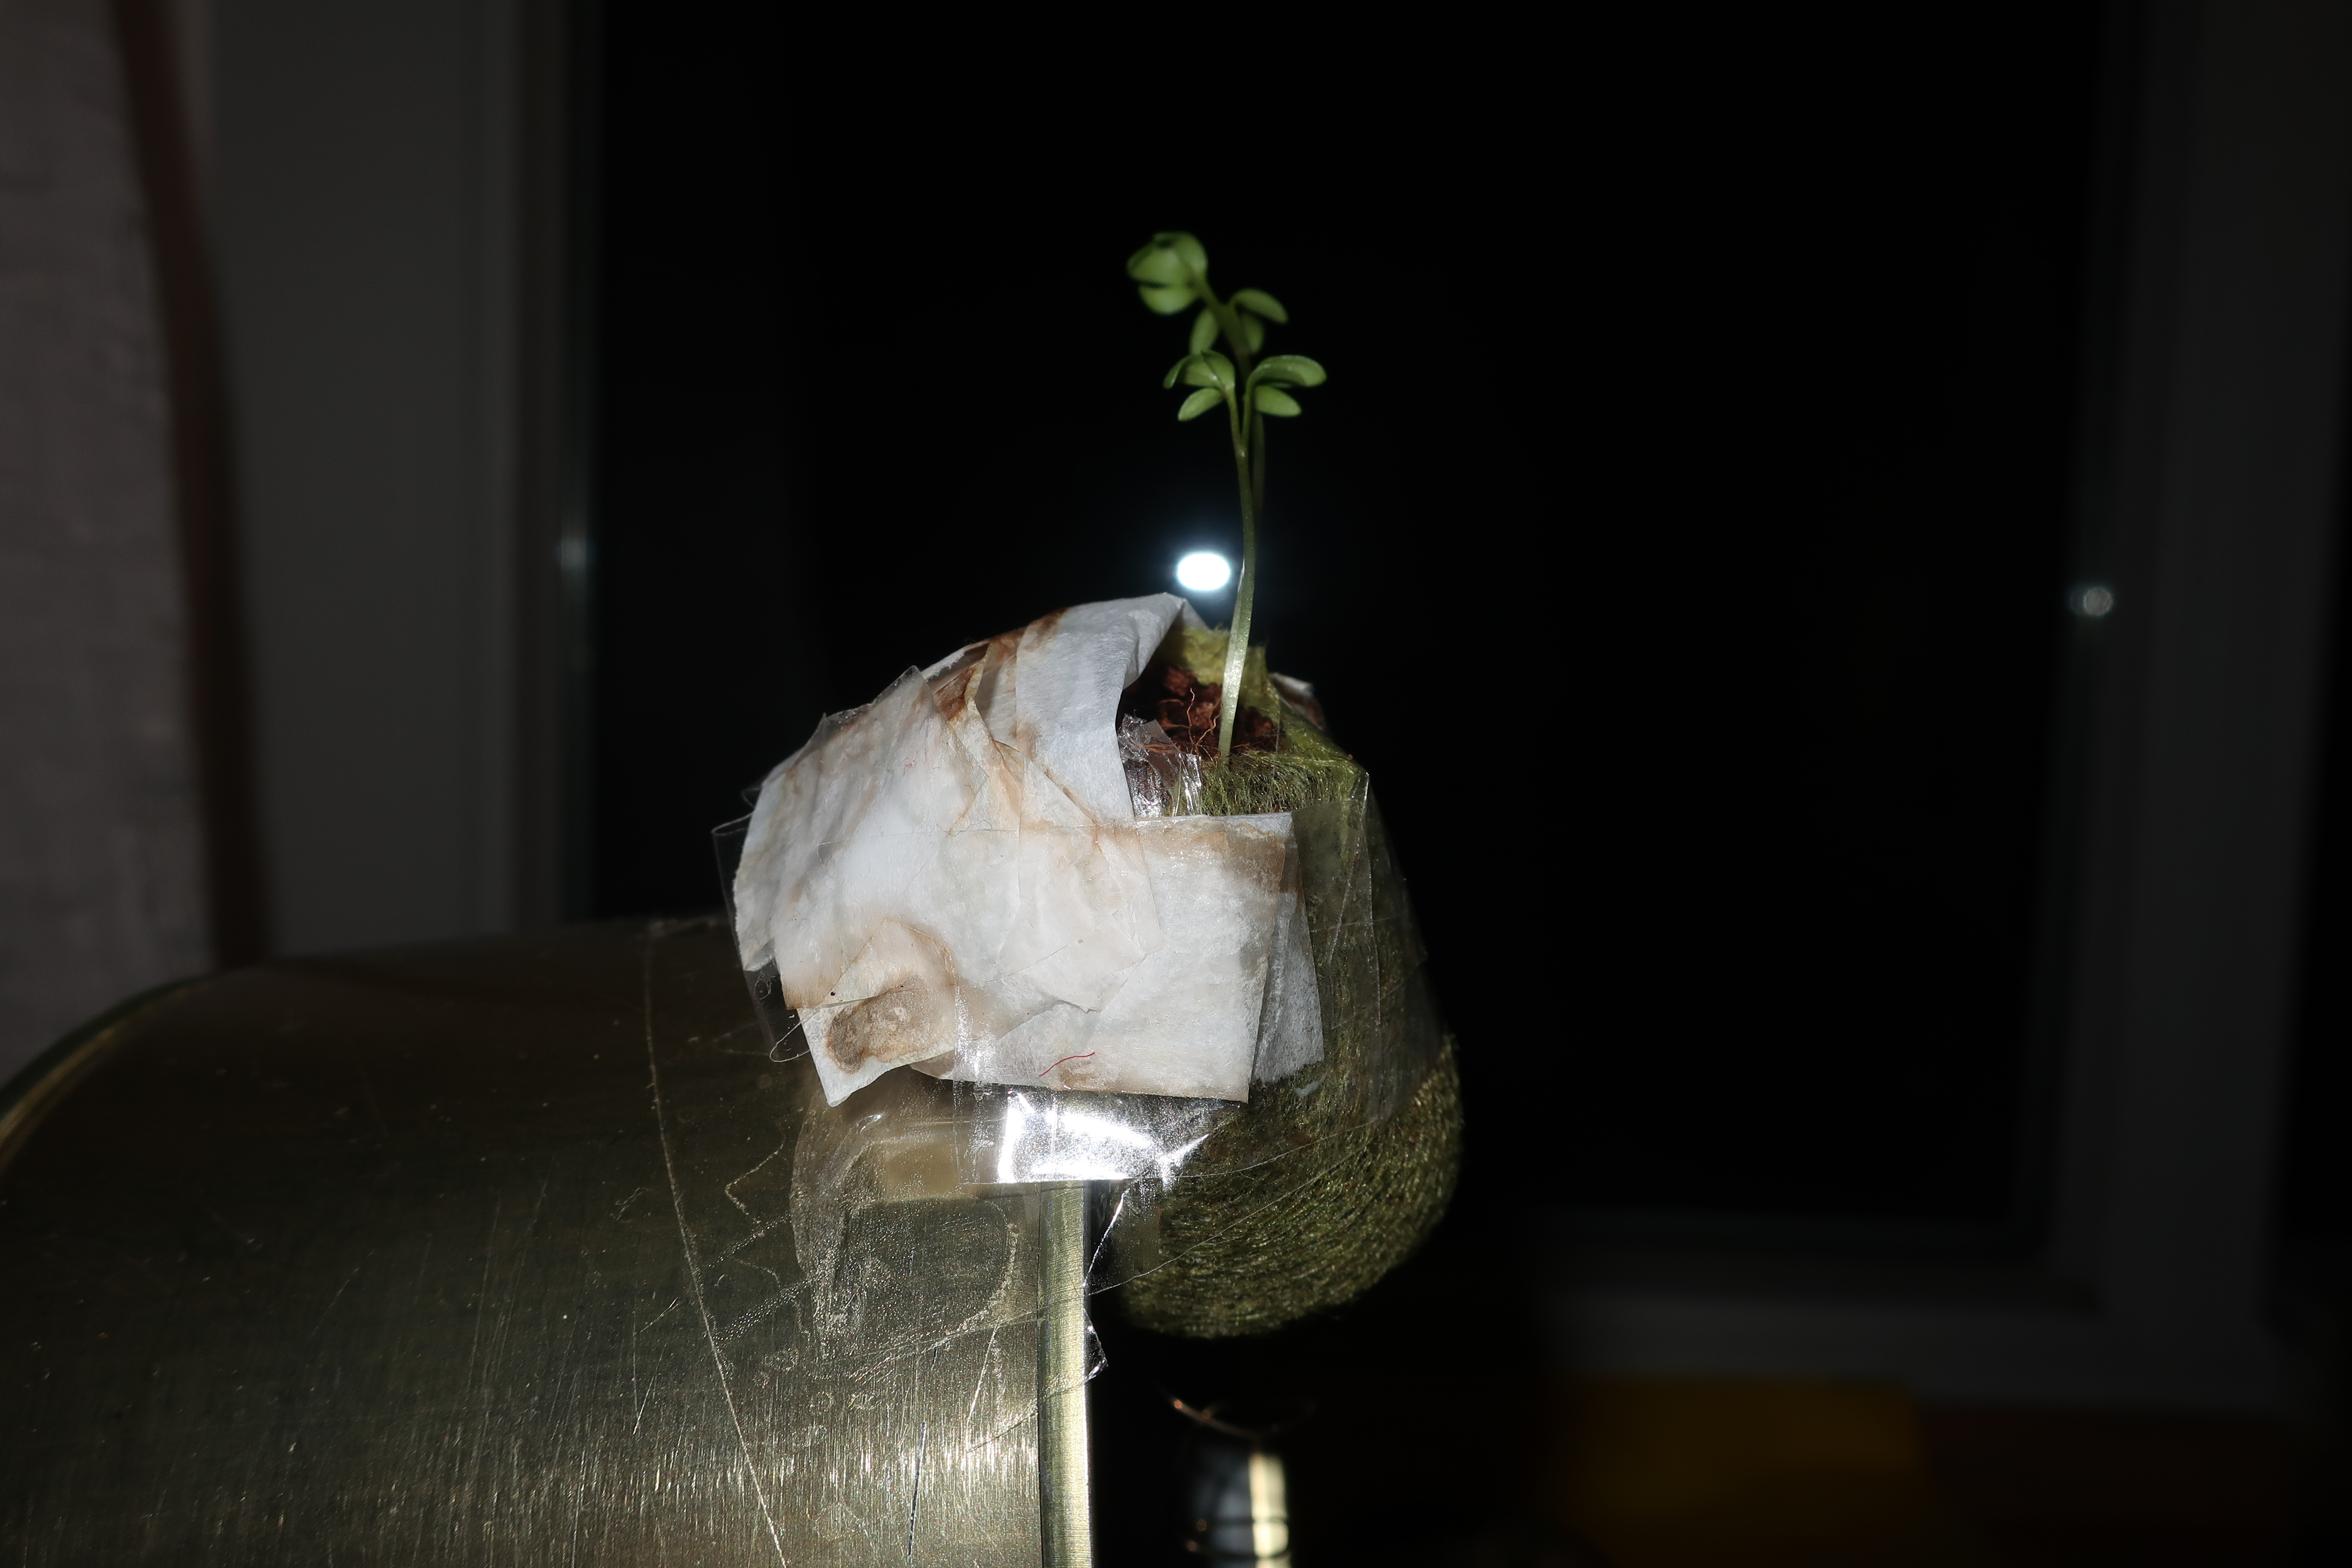
\includegraphics[width = .5\linewidth]{images/IMG_1114.JPG}
	\caption{Wieder senkrecht wachsende Sprösslinge \label{Foto 3}}
\end{figure}

6. Tag (02.06.18): Klinostat wurde wieder repariert und nochmal gestartet. Sprossen sind fast bis zu 3cm gewachsen.

\begin{figure}[H]
	\centering 
	\includegraphics[width = .5\linewidth]{images/IMG_1128.JPG}
	\caption{Sprösslinge bis zu 3cm \label{Foto 4}}
\end{figure}

7. Tag (03.06.18): Sprossen sind über 3cm gewachsen, aber sie haben sich langsamer gekrümmt ,wie in Abbildung \ref{Foto 5} zu sehen ist, als im ersten Durchlauf.

\begin{figure}[H]
	 \centering 
  \includegraphics [width =.5\linewidth]{images/IMG_1399.JPG}
  	\caption{Gravitrop reagierende Sprösslinge über zu 3cm. Kleinerer Spross gebogen, größerer Spross nur geneigt \label{Foto 5}}
\end{figure} 

 Auch in den Behältern haben die Sprösslinge sich gravitrop verhalten. Hier wird zum Veranschaulichen der quer gelegte Behälter abgebildet.
 In Abbildung \ref{Foto 6} befinden sich die Pflanzen im Originalzustand. Nach drei Tagen haben sie schon gravitrop reagiert und wachsen wieder senkrecht, wie in Abbildung \ref{Foto 7} zu erkennen ist.

\begin{figure}[H]
	\centering 
	\includegraphics [width =.5\linewidth]{images/IMG_1104.JPG}
	\caption{Sprösslinge am Anfang des Versuchs \label{Foto 6}}
\end{figure} 

\begin{figure}[H]
	\centering 
	\includegraphics [width =.5\linewidth]{images/IMG_1120.JPG}
	\caption{Sprösslinge am Ende des Versuchs \label{Foto 7}}
\end{figure} 


\section{Diskussion}

Pflanzen reagieren gravitrop, wenn ihre Lage verändert wird, ob sie kopfüber stehen, quer liegen oder drehen. Das haben die Resultate des Experiments  veranschaulicht. Es lässt sich ein Zusammenhang zwischen der Stärke der Krümmung und der Länge der Sprossen vermuten. In den anfänglichen Beobachtungen, als die Pflanzen unter 3cm Länge besitzen, reichen wenige Stunden (1-3 Stunden), bis die Pflanzen gravitrop reagieren. Ab einer Länge von 3cm lässt sich eine geringere Stärke der Krümmung über 24 Stunden feststellen.
In den Versuchen haben sich Pflanzen nicht komplett senkrecht gerichtet, sondern mehr zum Licht gewandt. Das liegt daran, dass Pflanzen sich immer zum Licht richten, um Photosynthese zu betreiben. Es kann angenommen werden, dass Pflanzen Gravitropismus und Phototropismus vereinen.
Es ist nicht auszuschließen, dass das Klinostat die Krümmung durch seine Geschwindigkeit beeinflussen kann.

  ist auch der Versuch mit dem Klinostat, denn ein weiterer Faktor, der die Krümmung beeinflussen könnte, ist die Geschwindigkeit. In diesem Experiment haben sich die Sprösslinge einmal pro Minute gedreht. Ob sie sich schneller krümmen, wenn die Geschwindigkeit erniedrigt wird oder ob sie sich nicht krümmen, weil der Klinostat die Pflanzen zu schnell dreht,kann als weiterführende Idee ausgeführt werden.


\chapter{Fazit und Ausblick}

Die Versuche haben nachgewiesen, dass es Gravitropismus in Pflanzen tatsächlich gibt und dass mehrere Faktoren diesen Prozess beeinflussen können. Es ist aber deutlich erkennbar, dass der Prozess des Gravitropismus aus drei Schritten besteht: Zuerst erfolgt die Reizaufnahme, dann die Signalübermittlung und zuletzt die Krümmung. Zwischen diesen Schritten erfolgen Prozesse, die teilweise noch nicht ganz geklärt sind, aber uns helfen den Gravitropismus besser zu verstehen. 

Diese Prozesse zu erforschen, die während der gravitropischen Reaktion erfolgen, ist eine der vielen Aufgaben mit der sich Naturwissenschaftler  heute befassen, da die gravitropische Fähigkeit der Pflanzen, zum Beispiel im Bereich der Landwirtschaft erforscht werden\parencite[343]{Chen1999}.
Hier anzuführen sind: Markus Braun; Zygmunt Hejnowicz; Rujin Chen, Elizabeth Rosen und Patrick H. Masson.


\printbibliography

\listoffigures

\chapter {Schlusserklärung}

Ich erkläre, dass ich die Seminararbeit ohne fremde Hilfe angefertigt und nur die im Literaturverzeichnis angeführte Quellen und Hilfsmitteln benützt habe.


Ort Datum Unterschrift des Schülers 

\end{document}
